%TODO: Arboles binarios
\begin{comment}
 Bibliografía utilizada aquí:
 
 \cite{Raghavendra84} -> Fault tolerance in Binary Tree Architecture
 
\end{comment}


\section{Árboles binarios}\label{sec:binary_tree}
El concepto de arquitecturas de árboles binarios es aplicable en el desarrollo de sistemas de 
computadoras jerárquicas, y sobre todo en computadoras de alta perfomance \citep{Raghavendra84}. 
Existen dos diferentes mecanismos de tolerancia a fallas \citep{Raghavendra84}:
\begin{enumerate}
 \item Esquemas con back up.
 \item Esquemas con degradación de perfomance.
\end{enumerate}

Teniendo en cuenta que estas arquitecturas son aplicadas principalmente en la construcción de 
circuitos VLSI\footnote{Del inglés, Very Large Scale Integration} \citep{Singh91}, se asume su 
aplicabilidad a arquitecturas de aviónica. 

La \ac{FT} y la perfomance de los sistemas dependen de las capacidades de las redes que se utilizan 
para la comunicación entre unidades de procesamiento \citep{Raghavendra84}. 

Un árbol binario está compuesto por nodos y enlaces (links). Existe un nodo central dónde se 
desprenden dos nodos hijos, estos se encuentran enlazados al nodo padre. Así recursivamente, se 
van generando dos nuevos hijos, por cada uno de los nodos. Los árboles binarios están divididos en 
niveles, que representa cada una de las generaciones de nodos.

Este tipo de topología tiene algunos problemas que la \ac{FT} debe hacer frente. En las 
arquitecturas basadas en árboles binario, existe una cierta probabilidad de que un nodo o un link 
falle \citep{Raghavendra84}. Las arquitecturas de árbol binario son en general físicamente 
estáticas. Por lo tanto, cualquier falla en uno de sus nodos (o links) demandaría una avería a 
nivel sistema, lo cual daría lugar a una pérdida de misión. Para ello se debe dotar a la 
arquitectura de un mecanismo de reconfiguración.

La tolerancia a fallas en arquitecturas binarias ya fueron estudiadas en profundidad en 
\cite{Hayes76}, \cite{Raghavendra84}, \cite{Singh91}. Para lograr \ac{FT} en estas arquitecturas se 
las deben diseñar con un número mínimo de nodos de backup y links redundantes, de modo tal de hacer 
frente cualquier punto de falla simple en la arquitectura. 

\subsection{Esquema de árbol binario con backups}
El esquema planteado por \cite{Raghavendra84} es similar al que se muestra en al Figura 
\ref{fig:binary_tree}. En este esquema se agregan nodos y links redundantes como técnica de \ac{FT}. 
Existe un nodo de backup por cada nivel del árbol.

\begin{figure}[h]
 \centering
 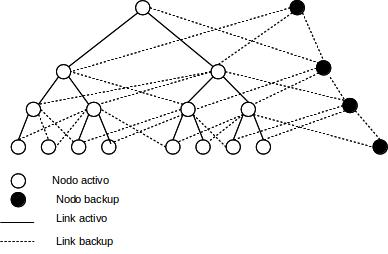
\includegraphics[scale=1]{images/Marco_teorico/binary_tree}
  \caption{Árbol binario de 4 niveles}  
\label{fig:binary_tree} 
\end{figure}

Esta arquitectura cuenta con una restricción, la cual indica que solo se puede tolerar una 
falla singular, por cada nivel de la arquitectura. Arquitecturas de este tipo, podrían tolerar más 
de una falla, sólo si se dan en diferentes niveles del árbol \citep{Raghavendra84}. Para agregar 
más tolerancia, se deberían agregar más redundancias.

Notese en la Figura \ref{fig:binary_tree} que cuando una unidad de procesamiento (nodo) falla, 
todos los links se deben reajustar hacia el nodo de la derecha. En este punto es importante 
mencionar, que ante esta situación se requiere una reconfguración a nivel de \ac{HW}, además de una 
reconfiguración a nivel de \ac{SW}. Es necesario algoritmos de ruteo dinámicos, de modo tal de 
conocer los nuevos caminos que intercomunican nodos, para mantener la operabilidad del sistema.  

\subsubsection{Estimación de la confiabilidad de un árbol binario con backup}
Se asume que la probabilidad de fallas de los links es muy baja en comparación con la de los nodos. 
Teniendo que el rate de falla es de $\lambda$, la confiabilidad  de un nodo es $R = e^{-\lambda 
t}$. También se sabe que un árbol binario con n niveles,  tiene $2^n - 1$ nodos en total. 
Entonces la confiabilidad de todo el sistema es: $$R_{nr} = R^{2^n - 1}$$

\cite{Raghavendra84} incluye en sus cálculos un factor de cobertura $c$, el cual es la probabilidad 
condicional de que se lleve a cabo una recuperación exitosa, luego de que una falla se haya 
detectado. Entonces la confiabilidad del sistema para una arquitectura de árbol binario con 
redundancias (un nodo backup por nivel) es el siguiente: $$R_{sys} = \prod_{k=0}^{n-1}{[R^{2k +1} + 
R^{2k}(1-R) + 2^kcR^{2k}(1-R)]}$$.

Simplificando: $$R_{sys} = R^{2n +1} \prod_{k=0}^{n-1}{[(2^kc+1) - 2^kcR]}$$

En la Figura \ref{fig:Reliability_binary_tree_4_levels}, se observa la confiabilidad de una 
arquitectura de árbol binario de 4 niveles, con una cantidad de $2^4 -1 = 15$ nodos. En color negro 
se grafica una arquitectura sin redundancia, mientras que en color rojo, azul y cyan, se muestra 
arquitecturas redundadas con diferentes $c$ (0.98, 0.99, 1, respectivamente). 

\begin{figure}[h]
 \centering
 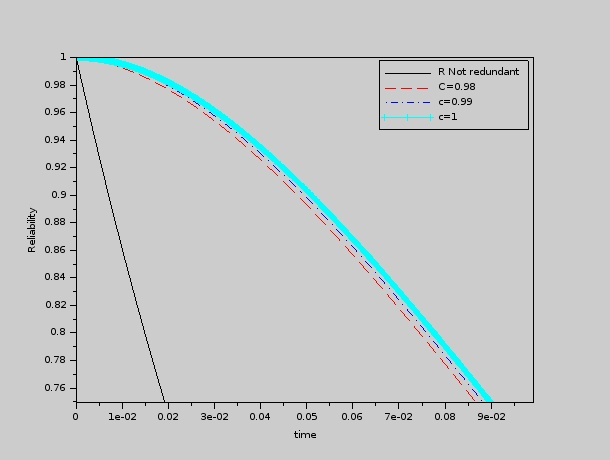
\includegraphics[scale=0.5]{images/Marco_teorico/Reliability_binary_tree_4_levels.jpg}
  \caption{Confiabilidad con respecto al tiempo de una arquitectura de árbol binario de 4 niveles}  
\label{fig:Reliability_binary_tree_4_levels} 
\end{figure}

Con esto podemos indicar, como es de esperarase, una arquitectura de árbol binario redundanda 
permite mantener un alto nivel deseable de confiabilidad, durante un mayor lapso de tiempo, a 
diferencia de un sistema no redundando. También se puede concluir que con un factor de cobertura $c$
más próximo a uno, maximiza los niveles de confiabilidad con respecto al tiempo. 

%\subsubsection{Extensión de la arquitectura con backup}

%\subsection{Esquema de árbol binario con degradación de perfomance}
